\begin{figure}[h!]
  \centering
  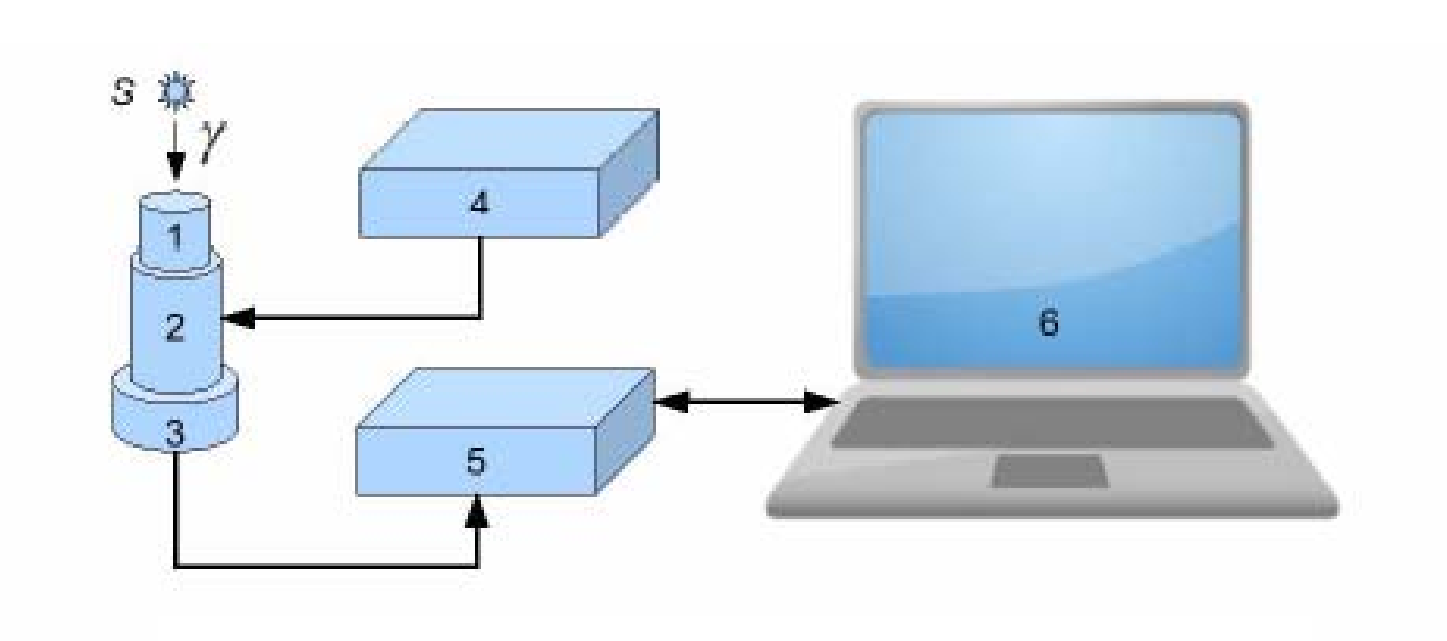
\includegraphics[width=0.8\linewidth]{pic6.png}
  \caption{Принципиальная блок-схема спектрометра}
  \label{pic:spectrometer}
\end{figure}

Принципиальная блок-схема гамма-спектрометра, изучаемого в данной работе,
показана на рис. \ref{pic:spectrometer}. На этом рисунке: 1 -- сцинтиллятор, 2
-- ФЭУ, 3 -- предусилитель импульсов, 4 -- высоковольтный блок питания для ФЭУ,
5 -- блок преобразования аналоговых импульсов с ФЭУ в цифровой код (АЦП), 6 --
компьютер для сбора данных, их обработки и хранения. ФЭУ со сцинтиллятором и
блоком питания установлены на отдельной подставке. В нашей работе на разных
установках (стендах) в качестве сцинтиллятора используются кристаллы NaI(Tl) с
размерами $\diameter $ $45 \times 50$ мм и $\diameter$ $20 \times 25$.